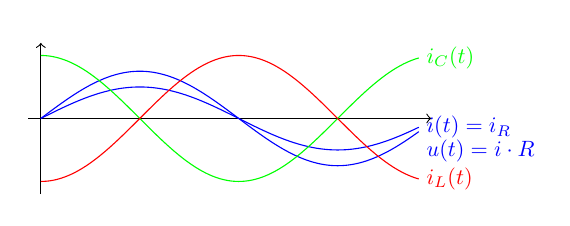
\begin{tikzpicture}[transform shape, scale=0.8, domain=0:6]
	
	\draw[->] (-0.2,0) -- (6.2,0) node[right] {};
	\draw[->] (0,-1.2) -- (0,1.2) node[above] {};
	\draw[color=blue, samples=150]   plot (\x,{0.5*sin(\x r)})   node[right]
	{$i(t)=i_R$};
	\draw[color=blue, samples=150]   plot (\x,{0.75*sin(\x r)})   node[below right]
	{$u(t)=i\cdot R$};
	\draw[color=green, samples=150]   plot (\x,{cos(\x r)})   node[right]
	{$i_C(t)$};
	\draw[color=red, samples=150]   plot (\x,{-1*cos(\x r)})  
	node[right] {$i_L(t)$};
\end{tikzpicture} 